\begin{figure}[htbp]
  \centering
  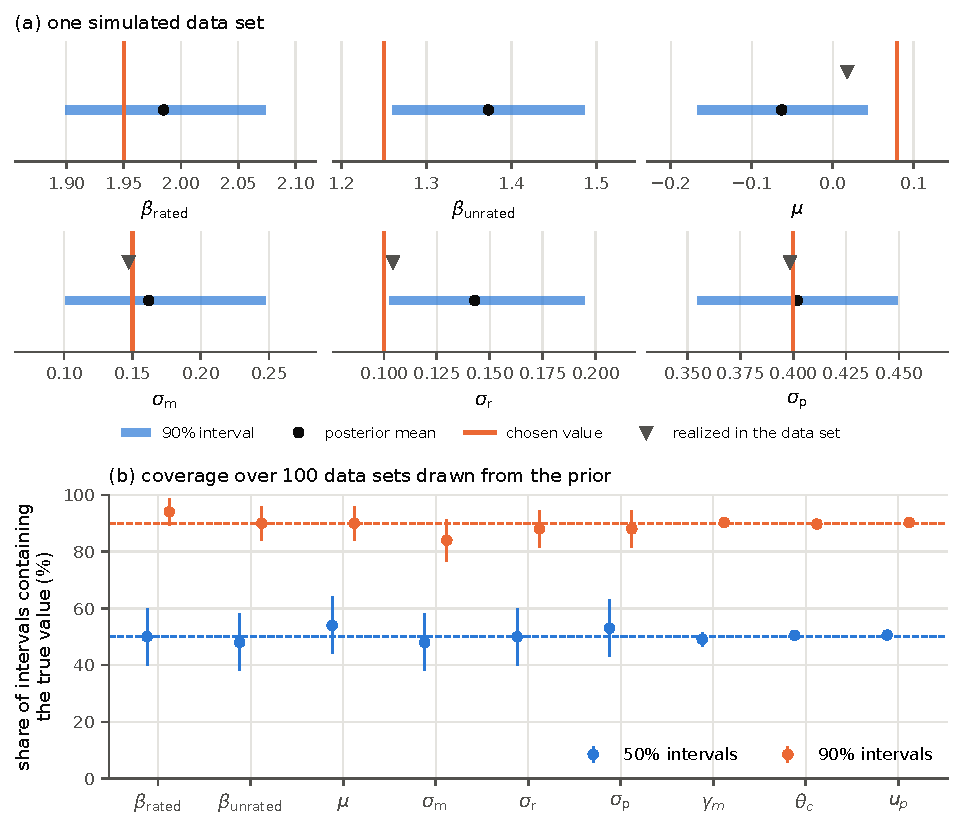
\includegraphics[width=\linewidth]{validation_full.pdf}
  \caption{Validation of the final model on simulated games, with the real rating gaps, rated status, pairs and players and the results drawn from the model. (a): one data set simulated with chosen values (orange lines); the posterior mean (black) and central 90\% interval (blue). The spreads and $\mu$ describe effects drawn once per data set, so the gray triangles mark the values realized in this data set, which the posterior targets. Over 40 data sets simulated with the same values, the slopes, $\mu$ and $\sigma_{\mathrm{p}}$ show no bias, but $\sigma_{\mathrm{r}}$ is overestimated by 0.049 on average (standard error 0.002) and $\sigma_{\mathrm{m}}$ by 0.040 (0.006): the $\text{Gamma}(1, 0.05)$ prior on the precisions puts less than 1\% of its mass on a spread as small as 0.10, and with few games per pair the data do not fully override it. (b): share of the 50\% and 90\% intervals that contain the true value, with $\pm 2$ standard errors, over 100 data sets whose parameters are drawn from the prior; for $\gamma_m$, $\theta_c$ and $u_p$ the share is over all first moves, pairs or players of all data sets. The shares match the nominal levels, as they must when the sampler is correct, whatever the prior.}
  \label{fig:validation_full}
\end{figure}
